We have evaluated two main areas;
\begin{itemize}
	\item The functional solidity --- using log files and JUnit~\cite{junit} tests
	\item The front-end usability --- using the Think Aloud Protocol
\end{itemize}

Clearly, both areas are important for a successful software system. 

\section{Functional Solidity}\label{policy-engine-system-evaluation}
JUnit tests are structured, assertable software tests that ensures that the software behaves as expected. Of course TDD\footnote{Test Driven Development} --- which we employed using the development of the core functionality --- has it's limits, mainly with regards to the quality of the written tests. The JUnit test accounts for the low level implementation tests.

On a higher abstraction level, we employes log files for testing. A log file is being generated at runtime, and has been integrated into (amongst other areas) the expression language. An example; we already know a certain policy's expected behavior (because we defined it ourselves) --- then we make sure that the policy is executed by the policy engine, and after the successful execution we carefully study the log file and compare it with the expected behavior. We find the log tests a natural selection on top of the more low level automated JUnit tests. It gave us a sense of extra security in regards to the behavior of the policy engine.

\subsection{Log Testing}
\label{log-test}
We have logged system data which was important as to determine if the system was working correctly. Doing so we have been able to verify the behavioral results and to discover bugs in our implementation --- which we then iteratively corrected. 

We have also been using the log files for source code quality control. We verified our solution by cross-referencing every action during tests, and matched it with the actual data stored in the database.

One excerpt from the log file can be seen in figure \ref{fig:log}

\begin{figure}[ht]
\centering
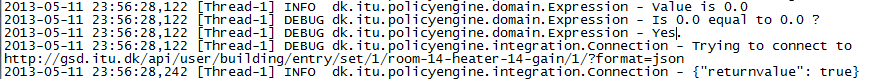
\includegraphics[width=\columnwidth]{images/logoutput.png}
\caption{An excerpt from the log file.}
\label{fig:log}
\end{figure}

\subsection{JUnit Testing}
To strengthen the solidity of the software, and minimize time used on debugging, we implemented a suite of JUnit Tests. An snippet of JUnit code can be seen in \ref{fig:junit-example}. Entering this test, the \textit{ROOM1\_HEATER} has been set to 1 and \textit{ROOM1\_TEMPERATURE} has been set to 26. The purpose is to see if the underlying expression language will set the \textit{ROOM1\_HEATER} to 0, which is should because the Expression's condition is using the \textit{Operator.GREATER\_THAN} along with a value of 25.
 
We have employed a sufficient amount of JUnit tests, to test all operators and both IfStatements (including nested capabilities) and SetStatements.

The result was that our IF-THEN-ELSE concept implementation performed as expected.

\begin{figure}[ht]
\centering
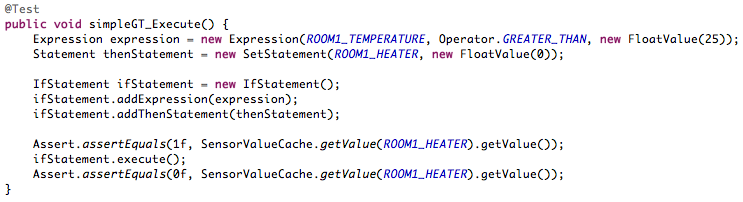
\includegraphics[scale=.5]{images/appendix-junit-example.png}
\caption{A snippet of a JUnit test.}
\label{fig:junit-example}
\end{figure}

\section{Usability Test}\label{sec:usability-test}
By using the Think Aloud Protocol we tested to uncover potential usability issues that needed solving.

To evaluate on the usability of our policy engine we decided to make a test with candidates outside of our development group. In general, when it come to "best practices of usability tests", the Think Aloud Protocol is considered one of the most valuable \cite{Nielsen1993}.

The Think Aloud Protocol is timewise inexpensive and easy to set and it also gives very valuable result from real-life scenarios.

\subsection{Think Aloud Protocol}
In a thinking aloud test, you ask test participants to use the system while continuously thinking out loud --- that is  simply verbalizing their thoughts as they move through the user interface, and take actions.

To run a basic thinking aloud usability study, 3 things are required:

\begin{itemize}
\item Recruit representative users.
\item Inform them of representative tasks to perform.
\item Avoid interference and let the users speak their actions.
\end{itemize}

We invited five people to a think aloud test. Research shows that having just five people will potentially uncover 80\% of all usability problems \cite{jakobnielsen2000fiveusers} as seen on \ref{fig:usabilitycurve}.

We conducted two think aloud tests, where the second test was aimed at fixing any usability issues found in the first iteration.

\begin{figure}[ht]
\centering
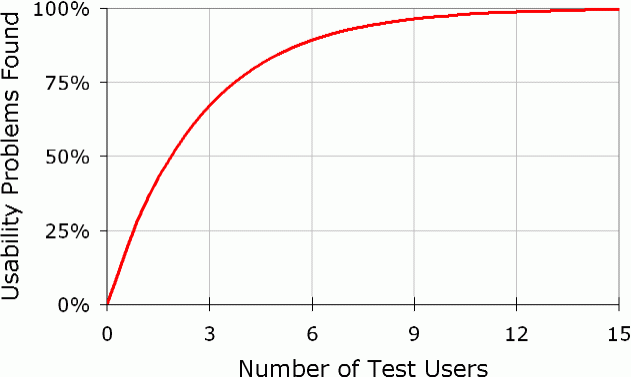
\includegraphics[width=\columnwidth]{usabilitycurve.png}
\caption{Usability test graph.}
\label{fig:usabilitycurve}
\end{figure}

The candidates is male and female students at ITU, between the age of 25 and 30. Some of them study software development and have a lot of knowledge in programming, others study digital design and knows more about human computer interaction and usability. However they all have web development in common.

\subsubsection{Tasks}
We arranged 7 tasks for the candidates to perform. Note however that the tests where held individually, but they were all given the same set of tasks. 
During the tests, candidates where only given one tasks at a time to focus on - using small tasks cards.

Before the test started we explained the purpose of the Policy Engine, and verbally gave them an example of a user case scenario.

We briefly introduced the participant with a map of the building and the rooms involved. We also gave an example list of sensor and actuator names to make them familiar with the elements involved, including basic knowledge of IF, AND, THEN statements and wild card operators. The questions were designed so that the candidates used all of the features available in the policy engine. The user interface contain a \textit{live auto complete function} so that the user can easily set a desired sensor/actuator without knowing the exact name. See section \ref{managing-policies} for more details.

The candidates where assigned the following tasks. 

\begin{framed}
Create a policy that turns the AC on in Room 1, 1. floor and name it "Cooling".
\end{framed}
The first task was designed to see how the user would try to create new policies - and how they would set name name.

\begin{framed}
Modify the "Cooling" policy you just created to affect both Room 1, 1. floor and Room 2, 2. floor.
\end{framed}
The second task was designed to see how the user handled modifying an existing policy.

\begin{framed}
Create a policy that turns on Blinds in all rooms for every floor in the building and name the policy "Sun".
\end{framed}
The third task was designed to see how the participant handled the "wildcard" feature.

\begin{framed}
Find and show the active policies just created.
\end{framed}
This fourth task showed how well the user handled the listing of active policies --- as this would likely be a typical reoccurring task for a building administrator.

\begin{framed}
Disable the policy named "Cooling" so that is no longer in function.
\end{framed}
The fifth task showed how well the user handle disabling/activating policies.

\begin{framed}
Delete the policy named "Sun".
\end{framed}
The sixth tasks showed the removal of policies.

\begin{framed}
To save energy the university wants to have the heating turned OFF automatically at 17:00. However this Wednesday around 19:00 - 22:00 an exclusive presentation is held in room number 5 on 1. floor.
You are asked to maintain a temperature at 21 degrees in that room throughout the presentation.
\end{framed}
The seventh task was designed to be more complex and the user was forced to work with expressions (AND) and operators such as larger than (\textgreater).

\begin{framed}
It is summertime and the overall temperature inside the building is rising. You are asked to keep the temperature at maximum 22 in all of the rooms in the building.
\end{framed}
% XXX --> The eight task was designed to be 

\begin{framed}
All afternoon between 12:00 and 16:00 the sun is at its peak. Therefore you are asked to set blinds ON in all the rooms on 1. floor and 2. floor - but only if the lights are ON.
\end{framed}
% XXX --> No description

\begin{framed}
The university wants to save energy. You are asked to make sure lights are automatic turned OFF at 17:00 in all the rooms, except from those on 0. Floor.
\end{framed}
% XXX --> No description

\subsubsection{Results and Comments}
\label{results-and-comments}
After every participant had gone through the think aloud test. We went through all their remarks. Some were the same, and those that were was combined into one.
For all the remarks, we made some comments as listed below --- including the actions we took to further improve the software.

\begin{quotation}
If there is a lot of policies - which I would expect there will be? Then I think the active policy list will be too long. I think it would make it difficult to find a specific (policy) if say you have a 100 policies.
\end{quotation}

The user is referring to the “Active Policy Site”, from which every active policy is listed underneath each other. The user finds that the site may force the user to do a lot of scrolling in order to find a specific policy.

Due to this remark we have implemented an expand function, which instead of listing all the content, in all of the listed policy, it only shows name, time and a button in the right hand corner, which if clicked expands the policy and reveals all of the content. This way the list will be much more compact and easier to go through. 

For future implementation we would also like to make a search function, from which the user is able to filter the policy by the search inputs. For example: name, or rooms effected  by the policy etc.
 
\begin{quotation}
I think it is difficult to see which one (rules) belong to what (expression).
\end{quotation}

The user is referring to the make up within a given policy. When a policy contains an IfStatement, the list of conditional expressions, and the then-clause and else-clause created some confusion. The user found that it was difficult to separate the different parts.

Due to this we implemented a color technique, which colorize the different parts. The conditional expressions now have a red background, while the content of the then-clause and else-clause has a green background.

In the second think aloud test, all participant expressed that they loved the coloring, and they found the overview better and easier to understand.

After the first think aloud test, we made changes to front-end design and we repeated the think aloud test, using the same set of tasks, to evaluate the impact of the changes.

After the second round of testing we only had some minor changes to do. But overall the participant where comfortable with the usability and had no further remarks.

We believe that there is always room for improvement, and we elaborate on this in the section \ref{subsec:improvements}.
%ATTENTION: Note: Insert results from think aloud test and write what we have learned from this